\documentclass[12pt]{article}
%\documentclass{article}
\usepackage{amsmath,amsthm,amssymb}
\usepackage{enumerate}

\usepackage[english]{babel}
 \usepackage{graphicx}
 \usepackage[usenames,dvipsnames,svgnames,table]{xcolor}
\usepackage{palatino}

\usepackage{fancyhdr}
\pagestyle{fancy}
\fancyhf{}
\rhead{Instructor: David Dobor}
\lhead{CIS 2033, Spring 2017, Homework 1}
\rfoot{Page \thepage}


\newenvironment{question}[2][Question]{\begin{trivlist}
\item[\hskip \labelsep {\bfseries #1}\hskip \labelsep {\bfseries #2.}]}{\end{trivlist}}
\newenvironment{answer}[2][Answer]{\begin{trivlist}
\item[\hskip \labelsep {\bfseries #1}\hskip \labelsep {\bfseries #2.}]}{\end{trivlist}}

\begin{document}

\subsection*{\centering{Homework 1 }}
\centering\textcolor{teal}{( Due at 11 AM Thursday, January 19 )}
\vspace{5mm}


 \begin{question}{1} Let $E$ and $F$ be two events in a sample space for which $P(E) = 1/4, P(F) = 1/2,$ and $P(E \cap F) = 1/6$. What is $P(E \cup F)$? 
\end{question} 

\vspace{5mm}


 \begin{question}{2} Let $A$ and $B$ be two events for which one knows that the probability that at least one of them occurs is 2033/3302. What is the probability that neither $A$ nor $B$ occurs? Hint: use one of DeMorgan's  laws: $A^c \cap B^c = (A \cup B)^c$ 
\end{question} 


\vspace{5mm}

\begin{question}{3} Consider a sample space that is the rectangular region
$[0, 1] \times [0, 2]$, i.e., the set of all pairs $(x, y)$ that satisfy $0 \leq x \leq 1$ and $0 \leq y \leq 2$.
 Consider a "uniform" probability law, under which the probability of an event is half of the area of the event. 
 Find the probability of the following events:
 \begin{enumerate}[(a)]
 \item The two components $x$ and $y$ have the same values.
 \item The value, $x$, of the first component is smaller than or equal to the value, $y$, of the second component.
  \item The value $x^2$ is smaller than or equal to the value of $y$. 
 \end{enumerate}

\end{question} 

\pagebreak


 \begin{question}{4} We toss a coin three times and write down the sample space for this experiment:
 $$\Omega = \{ HHH, THH,HTH,HHT, TTH, THT,HTT, TTT \}$$
 where $T$ stands for tails and $H$ for heads.
 

\begin{enumerate}[(a)]
\item 
 Write down the set of outcomes corresponding to each of the following
events:
\begin{itemize}
 \item $A:\ \ $``we throw tails exactly two times.''
 \item $B:\ \ $  ``we throw tails at least two times.''
 \item $C:\ \ $  ``tails did not appear \emph{before} a head appeared.”''
 \item $D:\ \ $  ``the first throw results in tails.''
 \end{itemize}
 \item What is the probability that event $A$ occurs?
 \item Look back at your answer in part (b). Can your answer be correct? How so? What assumptions did you make to compute $P(A)$?
 \item Can you compute the probability of event $B$ by making the assumption that all outcomes of the experiment are equally likely? If you answered 'yes', please compute it; if you answered 'no', please explain why?
 \item Write down the set of outcomes corresponding to each of the following events:
 $$ A^c, \ \ A \cup (C \cap D), \ \  A \cap D^c. $$
 \end{enumerate}
 
\end{question} 

\vspace{5mm}


 \begin{question}{5} Let $A$, $B$, and $C$ be disjoint subsets of the sample space. For each one of the following statements, determine whether it is true or false. Note: "False" means "not guaranteed to be true."

\begin{align}
&P(A) + P(A^c) + P(B) = P(A \cup A^c \cup B) \\
&P(A) + P(B) \leq 1 \\
&P(A^c) + P(B) \leq 1 \\
&P(A \cup B \cup C) \geq P(A \cup B)
\end{align}
\end{question} 

\vspace{5mm}

 \begin{question}{6} Prove that if events $A$ and $B$ are such that $A \subseteq B$, then $P(A) \leq P(B)$. Do events $A$ and $B$ from question 4 satisfy the conditions on $A$ and $B$ in this problem? 
 \end{question} 
 
\vspace{5mm}
 \begin{question}{7} You are rolling two tetrahedral dice. Let $X$ and $Y$ stand for the faces of the first and second die, respectively. 
We discussed the sample space of this experiment in class, and here it is depicted for your convenience again:
\begin{center}
 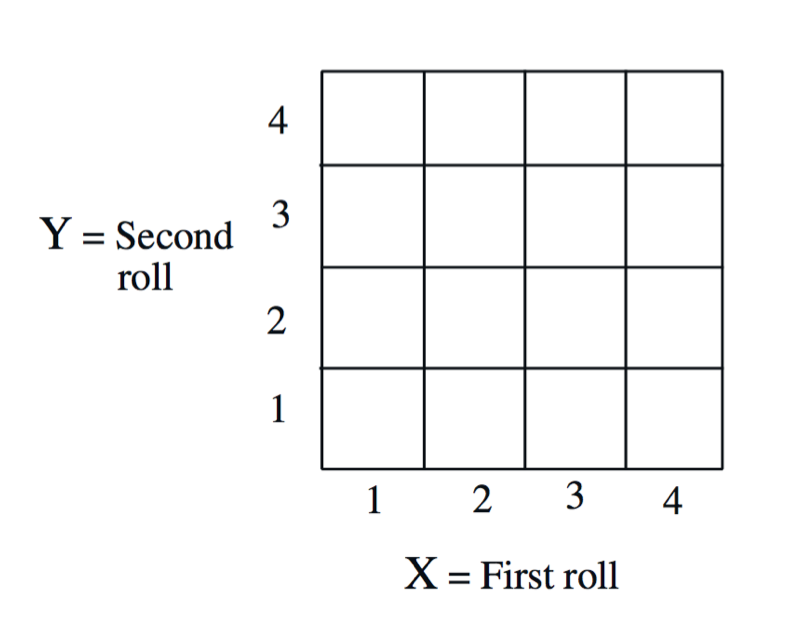
\includegraphics[scale=0.30]{TetraDie}
 \end{center}

Assume that all outcomes of your experiment are eqaully likely. 
\vspace{3mm}

Let $Z = \text{min }(X, Y)$, let  $ U = \text{max }(X, Y)$, and let $S$ be the sum of the faces showing, i.e. $S = X + Y$.

\begin{enumerate}[(a)]
 \item What is $P(Z = 3)$?
\item What is $P(U = 3)$?
 \item What is $P(S \text{ is even })$?
 \end{enumerate}
  \textit{Hint:} it may be illuminating to fill in the appropriate squares in this picture as you try to answer these questions.
 \end{question} 

\end{document}






















